\documentclass[paper=a4,DIV=12]{tmmlab}

\usepackage[polish]{babel}
\usepackage[T1]{fontenc}
\usepackage[utf8]{inputenc}
\usepackage{courier}
\usepackage{tgtermes,newtxtext,newtxmath}
\usepackage[pdftex,colorlinks,allcolors=blue]{hyperref}
\usepackage{natbib}

%%\everymath{\displaystyle}

\usepackage{bm}
\usepackage{amsmath,amsfonts}
\usepackage{mathtools}
\usepackage{graphicx}
\usepackage[titletoc,title]{appendix}
\usepackage{subcaption}
\usepackage{listings}
\usepackage{float}
\usepackage{tabularx}

\newcommand{\brm}[1]{\bm{\mathrm{#1}}}
\renewcommand{\arraystretch}{1.2}
\newcolumntype{L}[1]{>{\raggedright\arraybackslash}p{#1}}
\newcolumntype{C}[1]{>{\centering\arraybackslash}p{#1}}
\newcolumntype{R}[1]{>{\raggedleft\arraybackslash}p{#1}}

% commath provides \od, but the package is not available on my travis-ci setup
\newcommand{\od}[2]{\frac{\mathrm{d}#1}{\mathrm{d}#2}}
\newcommand{\odn}[3]{\frac{\mathrm{d}^{#1}#2}{\mathrm{d}{#3}^{#1}}}
\newcommand{\tod}[2]{\tfrac{\mathrm{d}#1}{\mathrm{d}#2}}
\newcommand{\todn}[3]{\tfrac{\mathrm{d}^{#1}#2}{\mathrm{d}{#3}^{#1}}}
% gensymb provides \degree command, but whole package for just one symbol?
\newcommand{\degree}{^{\circ}}

\lstset{%
  basicstyle=\footnotesize\ttfamily\selectfont,
  language=Matlab,
  inputencoding=utf8,
  extendedchars=true,
  frame=trBL
}

\newfloat{lstfloat}{htbp}{lop}
\floatname{lstfloat}{Listing}

\setcitestyle{numbers,square,comma}

\begin{document}

\serietitle{Laboratorum TMM}
\title{Ćwiczenie nr 11}
\subtitle{Analiza kinematyczna mechanizmu strugarki}
\author{Paweł Tomulik}
\date{}
\maketitle

\begin{abstract}
  Analiza kinematyczna przy użyciu metod teorii mechanizmów dotyczy często
  modeli wyidealizowanych, nie uwzględniających błędów wykonania czy stopnia
  zużycia. Badając rzeczywiste układy mechaniczne, nie sposób zignorować tych
  czynników, jak też błędów pomiarowych, którymi obarczony jest sam
  eksperyment. Analizę kinematyczną istniejącego mechanizmu można przeprowadzić
  stosując postępowanie doświadczalno-numeryczne. Jeden ze sposobów rozpoczyna
  się od zarejestrowania położeń badanego członu odpowiadających serii
  równo-odległych położeń członu napędzającego. Ponieważ zarówno sposób
  zadawania położeń członu napędzającego jak też metoda pomiaru położeń członu
  obserwowanego są obarczone błędem, stosuje się rachunek wyrównawczy w~celu
  jego zredukowania. Tak przetworzone wartości mogą być następnie użyte do
  wyznaczenia chwilowych prędkości i~przyspieszeń mechanizmu za pomocą wzorów
  interpolacyjnych.
\end{abstract}

\section{Wprowadzenie}
\label{sec:4S1JJ}

Przedmiotem badania jest model mechanizmu jarzmowego strugarki poprzecznej
(rys.~\ref{fig:TQIWQ}), umieszczony na tablicy-wsporniku~1. Zmianę położenia
modelu realizuje się za pomocą pokrętła~2 usytuowanego po przeciwnej (niż
model mechanizmu) stronie tablicy. Pokrętło to wyposażone jest we wskazówkę~3,
umożliwiającą odczytanie na kątomierzu~4 kąta obrotu korby~5,
umieszczonej na tym samym wałku co pokrętło~2. Korba~5 stanowi człon
napędzający modelu mechanizmu jarzmowego, składającego się ponadto z~wahacza~6,
łącznika~7, suwaka prowadnicy~8 i~suwaka wahacza~11. Zmianę
położenia suwaka prowadnicy~8 mierzy się za pomocą skali milimetrowej na
prowadnicy~9 i~noniusza na suwaku~8.
%%%%%%%%%%%%%%%%%%%%%%%%%%%%%%%%%%%%%%%%%%%%%%%%%%%%%%%%%%%%%%%%%%%%%%%%%%%%%%
\begin{figure}[htbp]
  \centering
  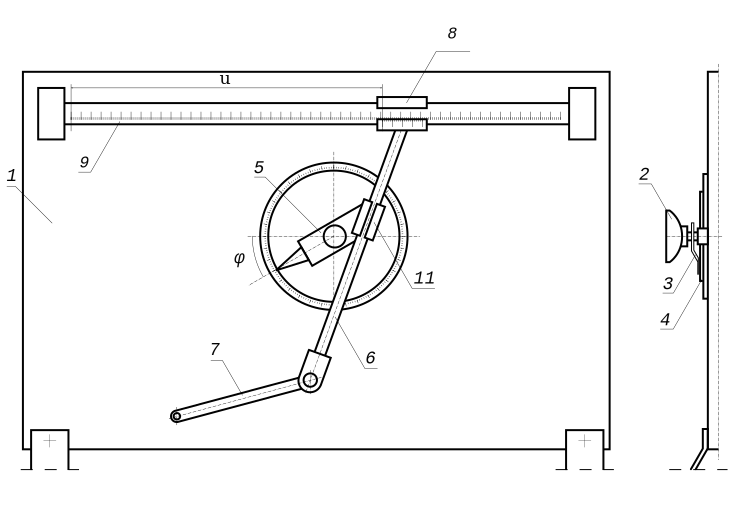
\includegraphics[width=0.9\textwidth]{lab11/strugarka}
  \caption{Model mechanizmu strugarki}
  \label{fig:TQIWQ}
\end{figure}
%%%%%%%%%%%%%%%%%%%%%%%%%%%%%%%%%%%%%%%%%%%%%%%%%%%%%%%%%%%%%%%%%%%%%%%%%%%%%%

Pod względem struktury, mechanizm składa się z~następujących członów: podstawy
(na rys.~\ref{fig:TQIWQ} elementy nr~1 oraz 9 należą do podstawy) i~pięciu
członów ruchomych. Są to: 5-korba, 6-wahacz, 7-łącznik, 8-suwak prowadnicy,
11-suwak wahacza.

Mechanizm jarzmowy tego typu był stosowany w~strugarkach poprzecznych do
konwersji ruchu obrotowego wału napędowego na ruch liniowy (posuwisto-zwrotny)
narzędzia. Przykłady takich obrabiarek przedstawiono na rys.~\ref{fig:27G0D}.
Pierwsze strugarki pojawiły się w~połowie XIX wieku i~były używane w~produkcji
mniej więcej do połowy XX wieku. Stosowane były np. do strugania płaszczyzn,
wykonywania uskoków, rowków pod wpusty klinowe czy rowków prowadnic
ślizgowych. Obecnie zostały wyparte przez inne obrabiarki oferujące podobne
możliwości (frezarki, szlifierki, przeciągarki, obrabiarki CNC).
%%%%%%%%%%%%%%%%%%%%%%%%%%%%%%%%%%%%%%%%%%%%%%%%%%%%%%%%%%%%%%%%%%%%%%%%%%%%%%
\begin{figure}[htbp]
  \centering
  \begin{subfigure}[b]{0.375\textwidth}
    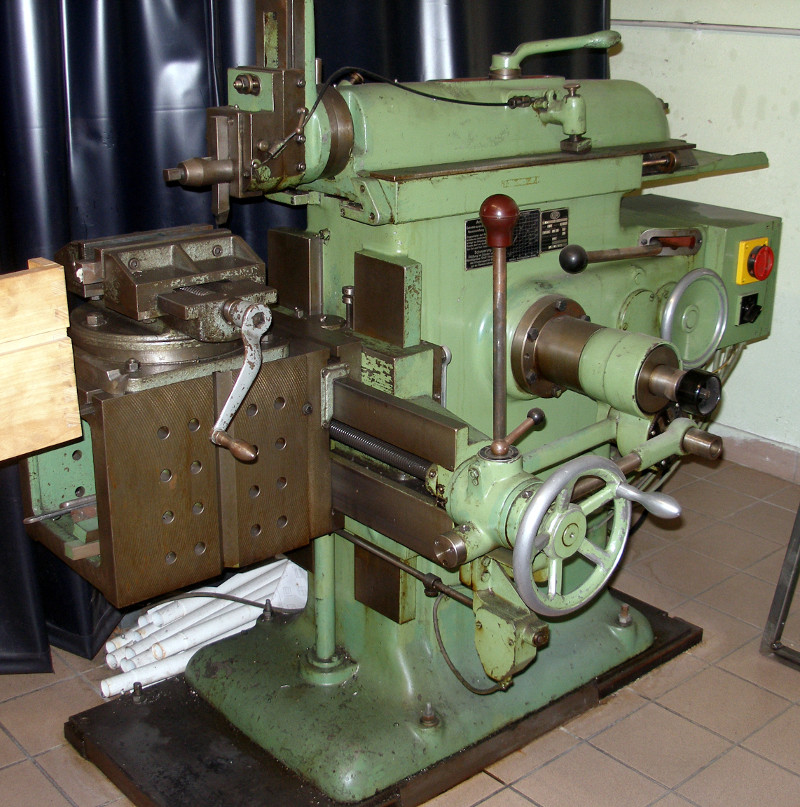
\includegraphics[height=0.26\textheight]{lab11/klopp375}
    \caption{Strugarka Klopp 375}
    \label{fig:ZGSAS}
  \end{subfigure}
  \begin{subfigure}[b]{0.5\textwidth}
    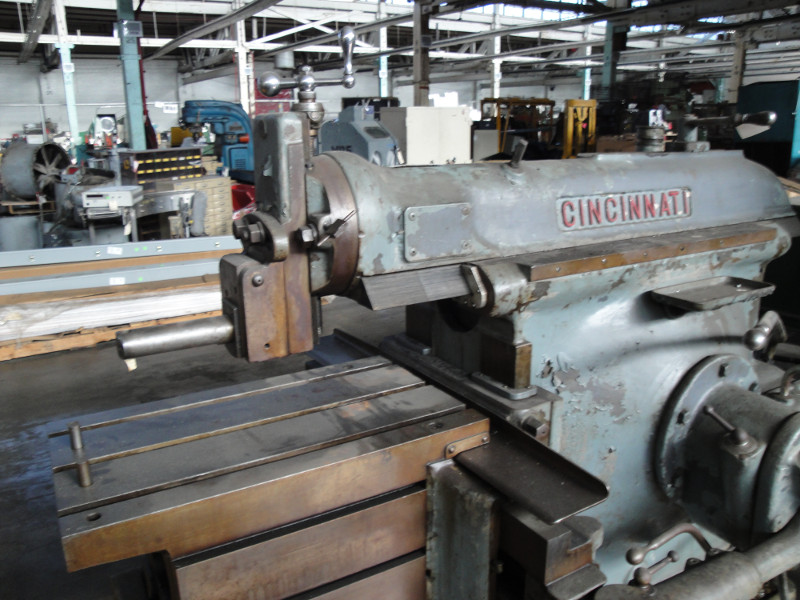
\includegraphics[height=0.26\textheight]{lab11/cincinnati}
    \caption{Strugarka Cincinnati}
    \label{fig:0W8XC}
  \end{subfigure}
  \caption{Przykłady strugarek poprzecznych (\url{https://wikipedia.org})}
  \label{fig:27G0D}
\end{figure}
%%%%%%%%%%%%%%%%%%%%%%%%%%%%%%%%%%%%%%%%%%%%%%%%%%%%%%%%%%%%%%%%%%%%%%%%%%%%%%

\section{Model kinematyczny mechanizmu strugarki}
\label{sec:V9TW6}

\paragraph{Struktura.} Schemat kinematyczny mechanizmu strugarki przedstawiono
na rys.~\ref{fig:4P8Y9}. Omawiany mechanizm, oprócz nieruchomej podstawy, ma
pięć członów ruchomych wymienionych we~wprowadzeniu (sekcja \ref{sec:4S1JJ})
oraz siedem par kinematycznych piątej klasy -- pięć obrotowych i~dwie
postępowe. Ruchliwość~$W$ mechanizmu określa się ze wzoru na ruchliwość
mechanizmów płaskich~\cite{oledzki:1987:podstawy}
%%%%%%%%%%%%%%%%%%%%%%%%%%%%%%%%%%%%%%%%%%%%%%%%%%%%%%%%%%%%%%%%%%%%%%%%%%%%%%
\begin{equation}
  W = 3 (n-1) - 2 p_5 - p_4 = 3 \cdot 5 - 2 \cdot 7 - 0 = 1,
  \label{eq:WGRDI}
\end{equation}
%%%%%%%%%%%%%%%%%%%%%%%%%%%%%%%%%%%%%%%%%%%%%%%%%%%%%%%%%%%%%%%%%%%%%%%%%%%%%%
gdzie $n$ jest liczbą członów (włącznie z~podstawą), $p_5$ liczbą par
kinematycznych piątej klasy (od\-bie\-ra\-ją\-cych dwa stopnie swobody
w~przypadku mechanizmów płaskich) i~$p_4$ liczbą par kinematycznych czwartej
klasy (odbierających jeden stopień swobody w~przypadku mechanizmów płaskich).
Zgodnie z~intuicją, mechanizm posiada jeden stopień swobody ($W = 1$).
%%%%%%%%%%%%%%%%%%%%%%%%%%%%%%%%%%%%%%%%%%%%%%%%%%%%%%%%%%%%%%%%%%%%%%%%%%%%%%
\begin{figure}
  \centering
  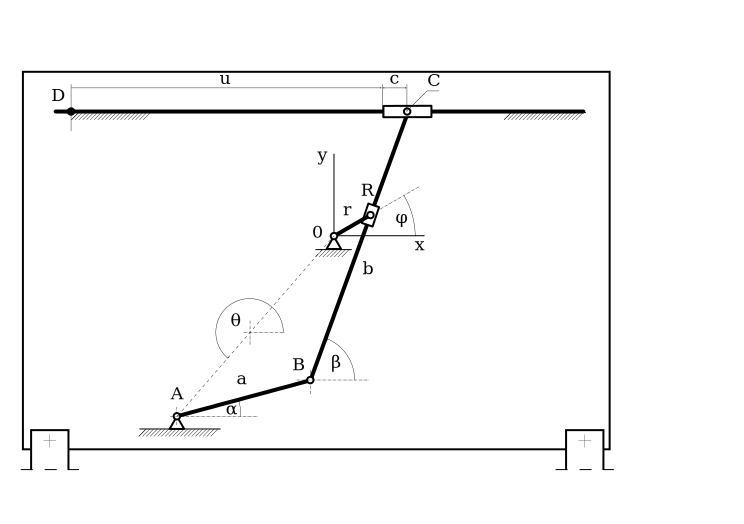
\includegraphics[width=0.9\textwidth]{lab11/strugarka-schemat}
  \caption{Schemat kinematyczny mechanizmu strugarki}
  \label{fig:4P8Y9}
\end{figure}
%%%%%%%%%%%%%%%%%%%%%%%%%%%%%%%%%%%%%%%%%%%%%%%%%%%%%%%%%%%%%%%%%%%%%%%%%%%%%%

\paragraph{Geometria.} Początek układu współrzędnych $x$-$y$ przyjęto w~punkcie
$O$ pokrywającym się z~osią obrotu korby~5. Istotne parametry geometryczne,
umożliwiające sformułowanie zadania kinematyki, to
%%%%%%%%%%%%%%%%%%%%%%%%%%%%%%%%%%%%%%%%%%%%%%%%%%%%%%%%%%%%%%%%%%%%%%%%%%%%%%
\begin{itemize}
  \item współrzędne $A_{(x)}$ i~$A_{(y)}$ punktu $A$ leżącego na osi obrotu łącznika 7,
  \item współrzędna $D_{(y)}$ prostej (,,poziomej'') po której porusza się środek obrotu suwaka 8,
  \item długość $r$ korby 5, długość $a$ łącznika 7 i~długość $b$ wahacza 6.
\end{itemize}
%%%%%%%%%%%%%%%%%%%%%%%%%%%%%%%%%%%%%%%%%%%%%%%%%%%%%%%%%%%%%%%%%%%%%%%%%%%%%%
Wymiar $c$ (odległość między osią obrotu suwaka 8 a~początkiem noniusza na
tym samym suwaku) i~współrzędną $D_{(x)}$ (współrzędna $x$ początku podziałki
prowadnicy 9) wprowadza się w~celu wyznaczenia wielkości $u$ obserwowanej
w~eksperymencie. Na rys.~\ref{fig:4P8Y9} punkt $D =
\left(D_{(x)},\,D_{(y)}\right)$. Wszystkie wymienione parametry są stałe, tzn.
nie zmieniają się na skutek ruchu członów modelu.

Zadanie kinematyki sformułowano w~dodatku \ref{sec:702WE}. Jego rozwiązanie
umożliwia wyznaczenie położeń~$u$ suwaka~8 odpowiadających zadanym położeniom
kątowym $\varphi$ korby~5 \emph{dla mechanizmu idealnego}. Ponadto, możemy
uzyskać teoretyczne wartości miejscowych prędkości $\dot u$ oraz przyspieszenia
$\ddot u$.

\paragraph{Funkcjonalność.} Omawiany mechanizm jarzmowy stosowano w~konstrukcji
strugarek poprzecznych ze względu na dwie kluczowe cechy. Po~pierwsze,
umożliwiał zamianę ruchu obrotowego na ruch posuwisto-zwrotny. Po~drugie, ruch
powrotny narzędzia trwał krócej niż ruch roboczy (ten drugi z~przyczyn
technologicznych musiał mieć ograniczoną prędkość). Umożliwiało to zachowanie
ograniczeń technologicznych procesu skrawania przy jednoczesnej redukcji
całkowitego czasu produkcji. Parametrem określającym ,,skuteczność''
mechanizmów tego typu jest \emph{współczynnik asymetrii ruchu}
%%%%%%%%%%%%%%%%%%%%%%%%%%%%%%%%%%%%%%%%%%%%%%%%%%%%%%%%%%%%%%%%%%%%%%%%%%%%%%
\begin{equation}
  e = \frac{T_r}{T_p},
  \label{eq:HMRCL}
\end{equation}
%%%%%%%%%%%%%%%%%%%%%%%%%%%%%%%%%%%%%%%%%%%%%%%%%%%%%%%%%%%%%%%%%%%%%%%%%%%%%%
gdzie $T_r$ jest czasem trwania ruchu roboczego a~$T_p$ czasem trwania ruchu
powrotnego przy stałej prędkości obrotowej korby. Korzyść z~zastosowania
mechanizmu jarzmowego oznacza $e > 1$.

Należy zauważyć, że wartość $e$ wynika wprost z~parametrów geometrycznych
mechanizmu. Eksperymentalnie można ją określić znajdując położenia korby
napędowej~5 odpowiadające położeniom zwrotnym suwaka prowadnicy~8
(rys.~\ref{fig:CMH6U})
%%%%%%%%%%%%%%%%%%%%%%%%%%%%%%%%%%%%%%%%%%%%%%%%%%%%%%%%%%%%%%%%%%%%%%%%%%%%%%
\begin{equation}
  e = \frac{\varphi_r}{\varphi_p}.
  \label{eq:LWY0U}
\end{equation}
%%%%%%%%%%%%%%%%%%%%%%%%%%%%%%%%%%%%%%%%%%%%%%%%%%%%%%%%%%%%%%%%%%%%%%%%%%%%%%
%%%%%%%%%%%%%%%%%%%%%%%%%%%%%%%%%%%%%%%%%%%%%%%%%%%%%%%%%%%%%%%%%%%%%%%%%%%%%%
\begin{figure}[htbp]
  \centering
  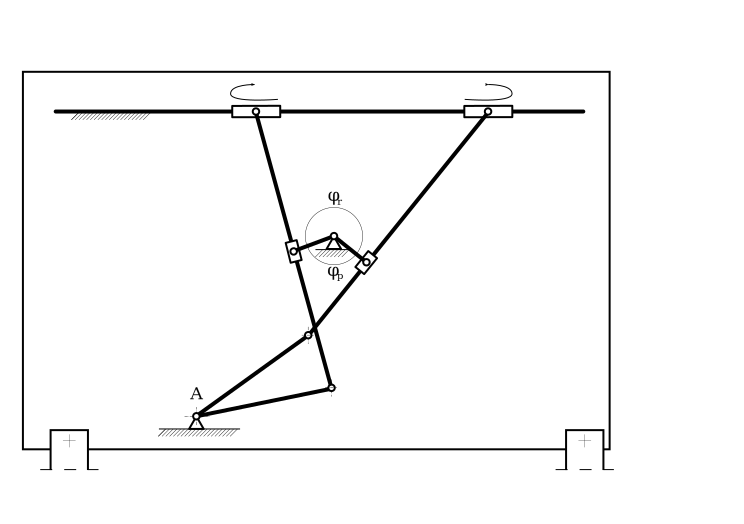
\includegraphics[height=0.4\textheight]{lab11/strugarka-zwrotniki}
  \caption{Mechanizm jarzmowy strugarki w~położeniach zwrotnych (rysunek
           poglądowy).}
  \label{fig:CMH6U}
\end{figure}
%%%%%%%%%%%%%%%%%%%%%%%%%%%%%%%%%%%%%%%%%%%%%%%%%%%%%%%%%%%%%%%%%%%%%%%%%%%%%%

Mechanizm jarzmowy nie jest jedynym, który umożliwia realizację ruchu
posuwisto-zwrotnego w~sposób asymetryczny. Innym przykładem jest asymetryczny
mechanizm korbowo-wodzikowy (rys.~\ref{fig:CMH6U}). Jednakże wartości $e$,
jakie można praktycznie uzyskać przy jego zastosowaniu, nie są
duże~\cite{oledzki:1987:podstawy}.
%%%%%%%%%%%%%%%%%%%%%%%%%%%%%%%%%%%%%%%%%%%%%%%%%%%%%%%%%%%%%%%%%%%%%%%%%%%%%%
\begin{figure}[htbp]
  \centering
  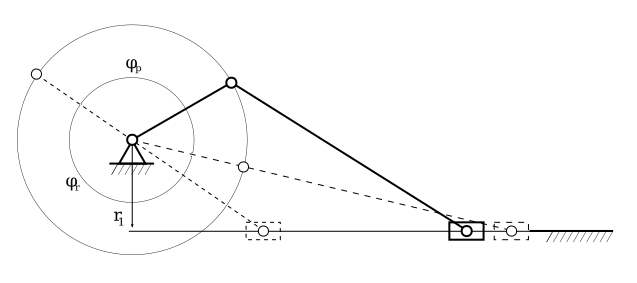
\includegraphics[width=0.8\textwidth]{lab11/korbowodzik-asymetryczny}
  \caption{Asymetryczny mechanizm korbowo-wodzikowy.}
  \label{fig:Z8R5Q}
\end{figure}
%%%%%%%%%%%%%%%%%%%%%%%%%%%%%%%%%%%%%%%%%%%%%%%%%%%%%%%%%%%%%%%%%%%%%%%%%%%%%%

\section{Rachunek wyrównawczy}
\label{sec:SZZY1}

Metoda rachunku wyrównawczego stosowana była powszechnie w~obliczeniach
geodezyjnych. Pomysł zastosowania jej do kinematyki mechanizmów zaproponował
J.~Oderfeld~\cite{oderfeld:1962:wstep}. W~tym kontekście, stosowany był przy
doświadczalnym określaniu przebiegów prędkości i~przyspieszeń w~mechanizmach.

W~przypadku idealnego mechanizmu jarzmowego, odpowiedni eksperyment można by
przeprowadzić mierząc położenia suwaka $u_i$ odpowiadające równo-odległym
położeniom korby napędzającej $\varphi_i = \Delta\varphi \cdot i$, a~następnie
wyznaczyć interesujące nas prędkości i~przyspieszenia stosując wzory różnicowe.
W~warunkach doświadczalnych pojawiają się jednak różne błędy pomiaru
i~obliczanie przyspieszeń ze~wzorów różnicowych staje się niecelowe -- uzyskane
przebiegi przyspieszeń mają niewiele wspólnego z~rzeczywistymi. Przy pomocy
odpowiedniej metody numerycznej można wtedy wprowadzić efekt ,,wygładzania''
przebiegów poszukując tzw. wartości wyrównanych a~następnie wyznaczyć prędkości
i~przyspieszenia bazując na przebiegach wyrównanych.

%%\subsection{Przebieg doświadczenia}
%%\label{sec:DQO4T}
%%
%%Doświadczenie rozpoczyna się od obrania liczby pomiarów $k$. Następnie
%%przeprowadza się je obracając pokrętło 2 każdorazowo o~przedział $\Delta\varphi
%%= \frac{360\degree}{k}$ i~rejestrując kolejne położenia suwaka 8. W~ten sposób
%%otrzymuje się ciąg surowych położeń $\left(u_i \right)$, gdzie $i= 1,2,\dots,k$.

\subsection{Przebieg obliczeń w~rachunku wyrównawczym}
\label{eq:R48E7}

W~metodzie tej wybiera się z~ciągu $\left(u_i\right)$, dla ustalonego wskaźnika
$i$, 11 wyrazów -- a mianowicie, oprócz samej $u_i$, 5 liczb poprzedzających
i~5 następujących. Następnie tworzy się z~nich kombinacje liniowe z~wagami
dobranymi w~sposób optymalny (patrz dodatek~\ref{sec:J0B6V}) i~podanymi
w~tablicy~\ref{tab:6MI34}.
%%%%%%%%%%%%%%%%%%%%%%%%%%%%%%%%%%%%%%%%%%%%%%%%%%%%%%%%%%%%%%%%%%%%%%%%%%%%%%
\begin{table}[htbp]
  \caption{Współczynniki stosowane w~rachunku wyrównawczym}
  \label{tab:6MI34}
  \centering
  \begin{tabular}{|c|c|c|c|c|c|c|c|c|c|c|c|}
    \hline
   $j$  & -5 & -4 & -3 & -2 & -1 &  0 &  1 &  2 &  3 &  4 & 5  \\\hline\hline
   $U_j$&    &    & -2 & +3 & +6 & +7 & +6 & +3 & -2 &    &    \\\hline
   $V_j$& -2 &+19 &-18 &-57 &-24 &  0 &+24 &+57 &+18 &-19 & +2 \\\hline
   $W_j$& +2 &-35 &+102&-33 &-24 &-24 &-24 &-33 &+102&-35 & +2 \\\hline
  \end{tabular}
\end{table}
%%%%%%%%%%%%%%%%%%%%%%%%%%%%%%%%%%%%%%%%%%%%%%%%%%%%%%%%%%%%%%%%%%%%%%%%%%%%%%
W~ten sposób powstają wielkości wyrównane (wzory~\eqref{eq:BNEHY})
%%%%%%%%%%%%%%%%%%%%%%%%%%%%%%%%%%%%%%%%%%%%%%%%%%%%%%%%%%%%%%%%%%%%%%%%%%%%%%
\begin{subequations}
  \label{eq:BNEHY}
  \begin{align}
    & \text{położenia} & & \hat{u}_i
        = \frac{1}{21} \sum_{j=-3}^{j=3} U_j u_{i+j} & & \text{[mm]},
    \label{eq:HOKXV}
    \\
    & \text{prędkości geom.} & & \hat{v}_i
        = \frac{1}{252} \sum_{j=-5}^{j=5} V_j u_{i+j} & & \text{[mm/przedział]},
    \label{eq:BQ71Z}
    \\
    & \text{przyspieszenia geom.} & & \hat{w}_i
        = \frac{1}{252} \sum_{j=-5}^{j=5} W_j u_{i+j} & & \text{[mm/przedział$^2$]}.
    \label{eq:7IT8Z}
  \end{align}
\end{subequations}
%%%%%%%%%%%%%%%%%%%%%%%%%%%%%%%%%%%%%%%%%%%%%%%%%%%%%%%%%%%%%%%%%%%%%%%%%%%%%%

Powyższe obliczenia można przeprowadzić w~środowisku Octave przy użyciu funkcji
\lstinline{conv} (listing~\ref{lst:NGICU}).
%%%%%%%%%%%%%%%%%%%%%%%%%%%%%%%%%%%%%%%%%%%%%%%%%%%%%%%%%%%%%%%%%%%%%%%%%%%%%%
\begin{lstlisting}[caption={Wyrównywanie współrzędnych w~programie Octave},label={lst:NGICU}]
  >> c = 1/21 * [-2, 3, 6, 7, 6, 3, -2]; % wspolczynniki wagowe
  >> nn = 3; % bierzemy trzy punkty na lewo i trzy na prawo
  >> ur = [ ... ]; % ur - wspolrzedne surowe (raw), z eksperymentu
  >> uu = cat(2,ur(end-(nn-1):end),ur,ur(1:nn)); % uu - wektor pomocniczy
  >> us = conv(uu,c,'valid'); % us - wspolrzedne wyrownane (smoothed)
\end{lstlisting}
%%%%%%%%%%%%%%%%%%%%%%%%%%%%%%%%%%%%%%%%%%%%%%%%%%%%%%%%%%%%%%%%%%%%%%%%%%%%%%
W~programie z~listingu~\ref{lst:NGICU} zastosowano pewną sztuczkę
(dołączanie elementów na początku i~końcu wektora \lstinline{ur}) ponieważ
przyjmujemy, że badana trajektoria ma charakter okresowy. Podobnie można
postąpić w~celu wyznaczenia prędkości i~przyspieszeń wyrównanych (wstawiając
właściwe współczynniki).

Dla zbadania dokładności oszacowań według powyższych wzorów, stosuje się
twierdzenie o~wariancji sumy niezależnych zmiennych losowych. W~tym celu
wyznacza się średnie odchylenie położeń surowych od wyrównanych
%%%%%%%%%%%%%%%%%%%%%%%%%%%%%%%%%%%%%%%%%%%%%%%%%%%%%%%%%%%%%%%%%%%%%%%%%%%%%%
\begin{equation}
  \bar{\sigma} = {\sqrt{\frac{1}{k} \sum_{i=1}^{k}{\left(u_i - \hat{u}_i\right)^2}}}.
  \label{eq:7Q65O}
\end{equation}
%%%%%%%%%%%%%%%%%%%%%%%%%%%%%%%%%%%%%%%%%%%%%%%%%%%%%%%%%%%%%%%%%%%%%%%%%%%%%%
Na tej podstawie można ustalić pasy tolerancji dla geometrycznych wielkości
wyrównanych. Mają one tę własność, że dla każdego wskaźnika $i$ obejmują
z~prawdopodobieństwem bliskim $95\%$  nieznane wielkości geometryczne zgodnie
z~tablicą~\ref{tab:IKYIL}.
%%%%%%%%%%%%%%%%%%%%%%%%%%%%%%%%%%%%%%%%%%%%%%%%%%%%%%%%%%%%%%%%%%%%%%%%%%%%%%
\begin{table}[htbp]
  \caption{Pasy tolerancji dla poszczególnych wielkości geometrycznych}
  \label{tab:IKYIL}
  \centering
  \begin{tabular}{|r|c|c|}
    \hline
    Wielkość geometryczna & Jednostka     & Pas tolerancji \\ \hline\hline
    Położenie             & mm            & $\hat{u}_i \pm 1,4143\bar{\sigma} $ \\ \hline
    Prędkość geom.        & mm/przedział  & $\hat{v}_i \pm 0,9237\bar{\sigma} $ \\ \hline
    Przyspieszenie geom.  & mm/przedział$^2$ & $\hat{w}_i \pm 1,6022\bar{\sigma} $ \\ \hline
  \end{tabular}
\end{table}

Wyznaczone dotychczas prędkości $\hat{v}_i$ i~przyspieszenia $\hat{w}_i$ są
tzw. wielkościami geometrycznymi, wyrażonymi w~jednostkach
$\tfrac{\text{mm}}{\text{przedział}}$ czy
$\tfrac{\text{mm}}{\text{przedział}^2}$. Aby uzyskać prędkości
$\dot{\hat{u}}_i$ i~przyspieszenia $\ddot{\hat{u}}_i$ wyrażone w~fizycznych
jednostkach, tj. $\tfrac{\text{mm}}{\text{s}}$
i~$\tfrac{\text{mm}}{\text{s}^2}$ należy zastosować wzory \eqref{eq:BH9VS}
i~\eqref{eq:0419L} przyjmując stałą, hipotetyczną prędkość kątową korby
$\dot{\varphi}$. W~eksperymencie $\Delta\varphi$ będzie wyrażone w~stopniach
$\degree$, zatem~$\dot{\varphi}$ należy podawać w~$\tfrac{\degree}{\text{s}}$.
Jeśli, jest potrzeba użycia prędkości obrotowej $n$ wyrażonej
w~$\tfrac{1}{\text{min}}$ (obrotach na minutę), to do wspomnianych wzorów
wstawia się $\dot{\varphi} = n \cdot \tfrac{6\degree}{\text{s}}$.

\section{Przebieg ćwiczenia}
\label{sec:DAUVI}

Podczas wykonywania niniejszego ćwiczenia student będzie posługiwał się
przygotowanym arkuszem kalkulacyjnym \texttt{rachwyr-clean.xls}, w~którym
zaimplementowano procedury rachunku wyrównawczego oraz estymacji błędów (pasy
tolerancji). Sam eksperyment sprowadza się do zebrania (w~czterech przejściach)
współrzędnych~$u_i$ suwaka odpowiadających równoodległym położeniom kątowym
korby~$\varphi_i$. Następnie należy wpisać je do arkusza.

\subsection{Opis arkusza kalkulacyjnego do rachunku wyrównawczego}
\label{sec:HPTQY}

Arkusz kalkulacyjny \texttt{rachwyr-clean.xls} zawiera następujące zakładki
\begin{itemize}
  \item \texttt{PAR} -- parametry metody (współczynniki rachunku wyrównawczego
    i~prędkość kątową $\omega = \dot{\varphi}$),
  \item \texttt{POM72} -- współrzędne zebrane w~eksperymencie z~$72$ punktami
    pomiarowymi ($\Delta\varphi = 5\degree$),
  \item \texttt{POM60} -- współrzędne zebrane w~eksperymencie z~$60$ punktami
    pomiarowymi ($\Delta\varphi = 6\degree$),
  \item \texttt{72}, \texttt{60}, \texttt{36}, \texttt{30}, \texttt{18},
    \texttt{15}, \texttt{9} -- wyniki obliczeń bazujących odpowiednio na
    $72$, $60$, $36$, $30$, $18$, $15$ i~$9$ punktach pomiarowych.
\end{itemize}

Zadaniem studenta jest uzupełnienie kolumn \texttt{u1[mm]} i~\texttt{u2[mm]}
w~zakładkach \texttt{POM72} i~\texttt{POM60} oraz wprowadzenie
odpowiedniej prędkości kątowej $\omega$ w~zakładce \texttt{PAR}. Pozostałe
komórki należy pozostawić bez zmian.

\subsection{Procedura pomiaru}
\label{sec:GCODS}

\begin{enumerate}
  \item Pobrać arkusz kalkulacyjny \texttt{rachwyr-clean.xls} i~zapisać go pod
    unikalną nazwą.
  \item Otworzyć w~Excelu (bądź innym adekwatnym programie) zapisany arkusz
    kalkulacyjny.
  \item Dokonać dwu serii pomiarów położeń suwaka odpowiadających położeniom
    korby $(0\degree, 5\degree, \dots, 355\degree)$, czyli dla $72$  punktów
    pomiarowych. Wyniki pomiaru wpisać w~kolumach \texttt{u1[mm]} (pierwsza
    seria) i~\texttt{u2[mm]} (druga seria) w~zakładce \texttt{POM72}.
  \item Dokonać dwu serii pomiarów położeń suwaka odpowiadających położeniom
    korby $(0\degree, 6\degree, \dots, 354\degree)$, czyli dla $60$  punktów
    pomiarowych. Wyniki pomiaru wpisać w~kolumach \texttt{u1[mm]} (pierwsza
    seria) i~\texttt{u2[mm]} (druga seria) w~zakładce \texttt{POM60}.
\end{enumerate}

\textbf{Uwaga!} -- w~sumie do wykonania jest $2 \times 72 + 2 \times 60 = 264$
pomiarów, co przy przeciętnym czasie pomiaru wynoszącym $10\,\text{sek}$ daje
ok. $45$ minut pracy nad samymi pomiarami. Wskazane jest sprawne i~szybkie
prowadzenie pomiarów aby zmieścić się w~wyznaczonym czasie.

\subsection{Interpretacja wyników}
\label{sec:M05YK}

W~zakładkach \texttt{72}, \texttt{60}, $\dots$, \texttt{9} arkusza
kalkulacyjnego znajdują się wyniki przetwarzania surowych współrzędnych
wprowadzonych w~arkuszach \texttt{POM72} i~\texttt{POM60}. Zakładki
\texttt{36}, \texttt{30}, \texttt{18}, \texttt{15} i~\texttt{9}  wybierają do
obliczeń np. co drugą bądź co czwartą wartość surową z~arkuszy \texttt{POM72}
bądź \texttt{POM60}. W~ten sposób realizowany jest sztucznie ,,dodatkowy
eksperyment'' z~mniejszą liczbą punktów pomiarowych, bez potrzeby ich
oddzielnego wprowadzania do arkusza.

Zakładki \texttt{72}, \texttt{60}, $\dots$, \texttt{9} zawierają wyniki
rachunku różnicowego (aproksymacja prędkości i~przyspieszeń suwaka metodą
różnic centralnych) oraz rachunku wyrównawczego (aproksymacja współrzędnych,
prędkości i~przyspieszeń metodą rachunku wyrównawczego). Wykresy umożliwiają
poglądową ocenę wynikowych przebiegów oraz graficzną reprezentację pasów
tolerancji. W~trakcie realizacji ćwiczenia należy się upewnić, że zgromadzone
dane nie zawierają błędów grubych.

\section{Przygotowanie sprawozdania}
\label{sec:FW8Q8}

W~sprawozdaniu należy zamieścić następujące informacje:
\begin{enumerate}
  \item Krótki opis wykonanego eksperymentu (maks. $\tfrac{1}{2}$ strony).
  \item Wykresy położeń ($mm$), prędkości ($mm/dz$) i~przyspieszeń
    ($mm/{dz}^2$) z~arkuszy \texttt{72}, \texttt{60}, $\dots$, \texttt{9}.
  \item Sporządzone samodzielnie: tabelę i~wykres przedstawiające szerokość
    pasów tolerancji $\Delta\hat{u}$ ($mm$), $\Delta\hat{v}$ ($mm/dz$ oraz
    $mm/s$) i~$\Delta\hat{w}$ ($mm/dz^2$ oraz $mm/s^2$) w~zależności od liczby
    punktów pomiarowych. Wykres powinien być skonstruowany następująco: oś
    pionowa $\rightarrow$ szerokość pasów tolerancji, oś pozioma
    $\rightarrow$ liczba punktów pomiarowych  $k$ (rozmiar eksperymentu).
  \item Sporządzone samodzielnie: tabelę i~wykres przestawiające wartości
    średniej odchyłki przyspieszeń obliczonych metodą rachunku wyrównawczego
    od~przyspieszeń obliczonych metodą rachunku różnicowego dla kolejnych
    wartości $k = 9, 18, \dots, 72$ liczby punktów pomiarowych
    \begin{equation}
      \epsilon_k = \sqrt{\frac{1}{k} \sum_{i=1}^k\left(\tilde{w}_i - \hat{w}_i\right)^2},
      \label{eq:INWGT}
    \end{equation}
    gdzie $\tilde{w}_i$ są przyspieszeniami obliczonymi metodą rachunku
    różnicowego. Należy przedstawić zarówno odchyłki wyrażone w $mm/dz^2$ jak
    i~$mm/s^2$. Oś pionowa $\rightarrow$ odchyłki, oś pozioma $\rightarrow$
    liczba punktów pomiarowych $k$.
  \item Określone samodzielnie: wartości kąta $\varphi$ odpowiadające
    położeniom zwrotnym suwaka, a~następnie wartości $\varphi_r$, $\varphi_p$
    oraz obliczony współczynnik asymetrii ruchu $e$
    wg~wzoru \eqref{eq:LWY0U}.
  \item Wnioski, głównie te dotyczące zachowania się błędów różniczkowania
    i~szerokości pasów tolerancji w~zależności od liczby punktów pomiarowych.
\end{enumerate}


\cleardoublepage

\begin{appendices}
  \section{Sformułowanie zadania kinematyki}
  \label{sec:702WE}
  Równania więzów, opisujące kinematykę mechanizmu strugarki, można zapisać
  na~kilka sposobów. Zapis przyjęty w~niniejszej instrukcji używa następującego
  zestawu współrzędnych kątowych (rys.~\ref{fig:4P8Y9})
  %%%%%%%%%%%%%%%%%%%%%%%%%%%%%%%%%%%%%%%%%%%%%%%%%%%%%%%%%%%%%%%%%%%%%%%%%%%%
  \begin{equation}
    \brm{q} \equiv \begin{bmatrix} q_{(1)} & q_{(2)} & q_{(3)} \end{bmatrix}^T
                    = \begin{bmatrix} \varphi & \alpha  & \beta   \end{bmatrix}^T.
    \label{eq:CBF4Z}
  \end{equation}
  %%%%%%%%%%%%%%%%%%%%%%%%%%%%%%%%%%%%%%%%%%%%%%%%%%%%%%%%%%%%%%%%%%%%%%%%%%%%

  \paragraph{Zadanie na położenie.}

  Rozwiązanie zadania na położenia umożliwi wyznaczenie położeń kątowych $\alpha$
  i~$\beta$ dla zadanego kąta obrotu korby $\varphi$. Obserwowaną
  w~eksperymencie współrzędną $u$ należy wtedy policzyć jako
  %%%%%%%%%%%%%%%%%%%%%%%%%%%%%%%%%%%%%%%%%%%%%%%%%%%%%%%%%%%%%%%%%%%%%%%%%%%%
  \begin{equation}
    u = \underbrace{A_{(x)} + a \cos{\alpha} + b \cos{\beta}}_{C_{(x)}} - c - D_{(x)}
    \label{eq:R3C32}
  \end{equation}
  %%%%%%%%%%%%%%%%%%%%%%%%%%%%%%%%%%%%%%%%%%%%%%%%%%%%%%%%%%%%%%%%%%%%%%%%%%%%
  Formułowanie zadań kinematyki rozpoczyna się zwykle od zapisania równań
  więzów. Równania więzów \emph{kinematycznych} dla mechanizmu strugarki można
  zapisać następująco
  %%%%%%%%%%%%%%%%%%%%%%%%%%%%%%%%%%%%%%%%%%%%%%%%%%%%%%%%%%%%%%%%%%%%%%%%%%%%%%
  \begin{equation}
    \brm{\Phi}(\brm{q}) \equiv \begin{bmatrix}
      A_{(y)} + a \sin{\alpha} + b \sin{\beta} - D_{(y)} \\
     -r \sin{(\varphi-\beta)} + a \sin{(\alpha - \beta)} + A \sin{(\theta - \beta)}
    \end{bmatrix} = \brm{0},
    \label{eq:V1TFC}
  \end{equation}
  %%%%%%%%%%%%%%%%%%%%%%%%%%%%%%%%%%%%%%%%%%%%%%%%%%%%%%%%%%%%%%%%%%%%%%%%%%%%%%
  przy czym przyjęto oznaczenie $A = \sqrt{A_{(x)}^2 + A_{(y)}^2}$ i~$\theta$:
  $A_{(x)} = A\cos{\theta}$, $A_{(y)} = A \sin{\theta}$.

  Pierwszy wiersz w~równaniu \eqref{eq:V1TFC} oddaje fakt, że $C_{(y)} =
  D_{(y)}$ (punkt $C$ porusza się po prowadnicy); drugi, że punkt $R$ porusza
  się wzdłuż odcinka $B$--$C$ (zob. dodatek~\ref{sec:F6O4D}). Powyższe więzy
  można też interpretować, w~kolejności, jako warunek domykania się czworoboku
  $A$-$B$-$C$-$D$ zrzutowany na kierunek osi $y$, oraz warunek domykania się
  czworoboku $A$-$B$-$R$-$O$ zrzutowany na kierunek prostopadły do $B$-$R$.

  Zadanie na położenie powstaje po dopisaniu do \eqref{eq:V1TFC} równania
  więzów \emph{kierujących}
  %%%%%%%%%%%%%%%%%%%%%%%%%%%%%%%%%%%%%%%%%%%%%%%%%%%%%%%%%%%%%%%%%%%%%%%%%%%%%%
  \begin{equation}
    \psiup(\brm{q},t) \equiv \varphi - \omega t = 0,
    \label{eq:XA8OD}
  \end{equation}
  %%%%%%%%%%%%%%%%%%%%%%%%%%%%%%%%%%%%%%%%%%%%%%%%%%%%%%%%%%%%%%%%%%%%%%%%%%%%%%
  gdzie $\omega = \operatorname{const}$ jest przyjętą prędkością kątową korby
  $[rad/s]$. Zadanie na położenie sprowadza się więc do rozwiązania
  nieliniowego układu równań
  %%%%%%%%%%%%%%%%%%%%%%%%%%%%%%%%%%%%%%%%%%%%%%%%%%%%%%%%%%%%%%%%%%%%%%%%%%%%%%
  \begin{equation}
    \brm{F}(\brm{q},t) \equiv \begin{bmatrix}
      \brm{\Phi}(\brm{q}) \\
      \psiup(\brm{q},t)
    \end{bmatrix}
    = \brm{0}
    \label{eq:B5Y8F}
  \end{equation}
  %%%%%%%%%%%%%%%%%%%%%%%%%%%%%%%%%%%%%%%%%%%%%%%%%%%%%%%%%%%%%%%%%%%%%%%%%%%%%%
  względem $\brm{q}$. Rozwiązanie numeryczne uzyskuje się przy użyciu
  iteracyjnej metody Newtona-Raphsona (lub podobnej). Procedury te zwykle
  działają sprawnie, jeśli dostarczy się im funkcję wyznaczającą macierz
  jakobianową $\brm{J}(\brm{q}) \equiv \partial{\brm{F}(\brm{q})}/\partial{\brm{q}}$.
  W~omawianym przypadku
  %%%%%%%%%%%%%%%%%%%%%%%%%%%%%%%%%%%%%%%%%%%%%%%%%%%%%%%%%%%%%%%%%%%%%%%%%%%%%%
  \begin{equation}
    \brm{J} = \begin{bmatrix}
      \brm{\Phi}_{\brm{q}} \\
      \boldsymbol{\psiup}_{\brm{q}}
    \end{bmatrix}
    \label{eq:YJI5X}
  \end{equation}
  %%%%%%%%%%%%%%%%%%%%%%%%%%%%%%%%%%%%%%%%%%%%%%%%%%%%%%%%%%%%%%%%%%%%%%%%%%%%%%
  oraz
  %%%%%%%%%%%%%%%%%%%%%%%%%%%%%%%%%%%%%%%%%%%%%%%%%%%%%%%%%%%%%%%%%%%%%%%%%%%%%%
  \begin{subequations}
    \label{eq:JSBPA}
    \begin{align}
    \brm{\Phi}_{\brm{q}}& = \begin{bmatrix}
      0 &
      a \cos{\alpha} &
      b \cos{\beta}
      \\
     -r \cos{(\varphi - \beta)} &
      a \cos{(\alpha - \beta)} &
      r \cos{(\varphi - \beta)} - a \cos{(\alpha - \beta)} - A \cos{(\theta - \beta)}
    \end{bmatrix},
    \\
    \boldsymbol{\psiup}_{\brm{q}} & = \begin{bmatrix}
      1 & 0 & 0
    \end{bmatrix}.
    \end{align}
  \end{subequations}

  \paragraph{Zadanie na prędkość.} Rozwiązanie zadania na prędkość umożliwi
  wyznaczenie chwilowych prędkości kątowych $\dot \alpha$ i~$\dot \beta$ dla
  zadanej konfiguracji $\brm{q}$ i~ustalonej prędkości korby $\omega$.
  Prędkość suwaka $\dot u$ należy wtedy policzyć jako
  %%%%%%%%%%%%%%%%%%%%%%%%%%%%%%%%%%%%%%%%%%%%%%%%%%%%%%%%%%%%%%%%%%%%%%%%%%%%
  \begin{equation}
    {\dot u} = - a \sin{\alpha} \cdot {\dot \alpha} - b \sin{\beta} \cdot {\dot \beta}.
    \label{eq:Y3EXW}
  \end{equation}
  %%%%%%%%%%%%%%%%%%%%%%%%%%%%%%%%%%%%%%%%%%%%%%%%%%%%%%%%%%%%%%%%%%%%%%%%%%%%
  Zadanie na prędkość ma postać układu równań liniowych (powstałych przez
  zróżniczkowanie~\eqref{eq:B5Y8F})
  %%%%%%%%%%%%%%%%%%%%%%%%%%%%%%%%%%%%%%%%%%%%%%%%%%%%%%%%%%%%%%%%%%%%%%%%%%%%
  \begin{equation}
    \brm{J} \brm{v} = - \brm{F}_t,
    \label{eq:1103T}
  \end{equation}
  %%%%%%%%%%%%%%%%%%%%%%%%%%%%%%%%%%%%%%%%%%%%%%%%%%%%%%%%%%%%%%%%%%%%%%%%%%%%
  które należy rozwiązać względem $\brm{v} = \begin{bmatrix} {\dot \varphi}
  & {\dot \alpha} & {\dot \beta} \end{bmatrix}^T$. Funkcja macierzowa
  $\brm{J}\left(\brm{q}\right)$ jest zdefiniowana wzorem
  \eqref{eq:YJI5X}, zaś pochodna $\brm{F}_t \equiv
  {\partial{\brm{F}}}/{\partial {t}}$ ma postać
  %%%%%%%%%%%%%%%%%%%%%%%%%%%%%%%%%%%%%%%%%%%%%%%%%%%%%%%%%%%%%%%%%%%%%%%%%%%%
  \begin{equation}
    \brm{F}_t = \begin{bmatrix}
      0 & 0 & - \omega
    \end{bmatrix}^T.
    \label{eq:6KPI4}
  \end{equation}
  %%%%%%%%%%%%%%%%%%%%%%%%%%%%%%%%%%%%%%%%%%%%%%%%%%%%%%%%%%%%%%%%%%%%%%%%%%%%

  \paragraph{Zadanie na przyspieszenie.} Rozwiązanie zadania na przyspieszenie
  umożliwi wyznaczenie chwilowych przyspieszeń kątowych ${\ddot \alpha}$
  i~${\ddot \beta}$ dla chwilowej konfiguracji $\brm{q}$ i~prędkości
  $\brm{v}$, przy założeniu, że przyspieszenie kątowe korby jest ${\ddot
  \varphi} = 0$. Przyspieszenie suwaka ${\ddot u}$ należy wtedy policzyć jako
  %%%%%%%%%%%%%%%%%%%%%%%%%%%%%%%%%%%%%%%%%%%%%%%%%%%%%%%%%%%%%%%%%%%%%%%%%%%%
  \begin{equation}
    {\ddot u} = -a \sin{\alpha} \cdot {\ddot \alpha} - b \sin{\beta} \cdot {\ddot \beta}
                -a \cos{\alpha} \cdot {({\dot \alpha})}^2
                -b \cos{\beta}  \cdot {({\dot \beta})}^2
    \label{eq:XUEF2}
  \end{equation}
  %%%%%%%%%%%%%%%%%%%%%%%%%%%%%%%%%%%%%%%%%%%%%%%%%%%%%%%%%%%%%%%%%%%%%%%%%%%%
  Zadanie na przyspieszenie ma~postać układu równań liniowych (powstałych przez
  zróżniczkowanie~\eqref{eq:1103T})
  %%%%%%%%%%%%%%%%%%%%%%%%%%%%%%%%%%%%%%%%%%%%%%%%%%%%%%%%%%%%%%%%%%%%%%%%%%%%
  \begin{equation}
    \brm{J} \brm{w} = - \od{\brm{J}}{t} \brm{v},
    \label{eq:U49AH}
  \end{equation}
  %%%%%%%%%%%%%%%%%%%%%%%%%%%%%%%%%%%%%%%%%%%%%%%%%%%%%%%%%%%%%%%%%%%%%%%%%%%%
  który należy rozwiązać względem $\brm{w} = \begin{bmatrix} \ddot{\varphi}
  & \ddot{\alpha} & \ddot{\beta} \end{bmatrix}^T$. Pochodna $\od{\brm{J}}{t}$
  wyraża się wzorem
  %%%%%%%%%%%%%%%%%%%%%%%%%%%%%%%%%%%%%%%%%%%%%%%%%%%%%%%%%%%%%%%%%%%%%%%%%%%%
  {\footnotesize\begin{equation}
    \od{\brm{J}}{t} = \begin{bmatrix}
       0 &
      -\dot{\alpha} a \sin{\alpha} &
      -\dot{\beta} b \sin{\beta}
      \\
       (\dot{\varphi}-\dot{\beta}) r \sin{(\varphi-\beta)} &
      -(\dot{\alpha}-\dot{\beta}) a \sin{(\alpha-\beta)} &
      -(\dot{\varphi}-\dot{\beta}) r \sin{(\varphi-\beta)}
        +(\dot{\alpha}-\dot{\beta}) a \sin{(\alpha-\beta)}
        - \dot{\beta} A\sin{(\theta-\beta)}
      \\
      0 & 0 & 0
    \end{bmatrix}.
    \label{eq:19DAI}
  \end{equation}}
  %%%%%%%%%%%%%%%%%%%%%%%%%%%%%%%%%%%%%%%%%%%%%%%%%%%%%%%%%%%%%%%%%%%%%%%%%%%%

  \section{Objaśnienie dotyczące równań więzów}
  \label{sec:F6O4D}
  Wyjaśnienia może wymagać drugie pośród równań więzów \eqref{eq:V1TFC}.
  Obserwując rys.~\ref{fig:4P8Y9} można zapisać warunek ograniczający ruch
  punktu $R$ do prostej przebiegającej przez punkty $B$ i~$C$
  %%%%%%%%%%%%%%%%%%%%%%%%%%%%%%%%%%%%%%%%%%%%%%%%%%%%%%%%%%%%%%%%%%%%%%%%%%%%
  \begin{equation}
    \frac{\sin{\beta}}{\cos{\beta}}
  = \frac{r\sin{\varphi} - \left(a\sin{\alpha} + A_{(y)}\right)}
         {r\cos{\varphi} - \left(a\cos{\alpha} + A_{(x)}\right)}.
    \label{eq:JT0OO}
  \end{equation}
  %%%%%%%%%%%%%%%%%%%%%%%%%%%%%%%%%%%%%%%%%%%%%%%%%%%%%%%%%%%%%%%%%%%%%%%%%%%%
  Lewa strona równania \eqref{eq:JT0OO} opisuje nachylenie odcinka $B$--$C$
  ($\tan{\beta}$). Prawa strona opisuje nachylenie odcinka $B$--$R$.
  Przekształcając powyższe równanie otrzymuje się
  %%%%%%%%%%%%%%%%%%%%%%%%%%%%%%%%%%%%%%%%%%%%%%%%%%%%%%%%%%%%%%%%%%%%%%%%%%%%
  \begin{equation}
    \sin{\beta}\left[r \cos{\varphi} - \left(a \cos{\alpha} + A_{(x)}\right)\right]
   -\cos{\beta}\left[r \sin{\varphi} - \left(a \sin{\alpha} + A_{(y)}\right)\right]
   = 0.
    \label{eq:KOLT5}
  \end{equation}
  %%%%%%%%%%%%%%%%%%%%%%%%%%%%%%%%%%%%%%%%%%%%%%%%%%%%%%%%%%%%%%%%%%%%%%%%%%%%
  Po skrupulatnym wymnożeniu wyrazów i~przyjęciu $A_{(x)} = A \cos{\theta}$,
  $A_{(y)} = A\sin{\theta}$
  %%%%%%%%%%%%%%%%%%%%%%%%%%%%%%%%%%%%%%%%%%%%%%%%%%%%%%%%%%%%%%%%%%%%%%%%%%%%
  \begin{equation}
  - r \left(\sin{\varphi} \cos{\beta} - \cos{\varphi}\sin{\beta}\right)
  + a \left(\sin{\alpha}\cos{\beta} - \cos{\alpha}\sin{\beta}\right)
  + A\left(\sin{\theta}\cos{\beta} - \cos{\theta}\sin{\beta}\right) = 0.
    \label{eq:6LMS9}
  \end{equation}
  %%%%%%%%%%%%%%%%%%%%%%%%%%%%%%%%%%%%%%%%%%%%%%%%%%%%%%%%%%%%%%%%%%%%%%%%%%%%
  Dla uzyskania drugiego równania \eqref{eq:V1TFC} pozostaje zaaplikować
  znane tożsamości trygonometryczne.

  \section{Dobór współczynników w~rachunku wyrównawczym}
  \label{sec:J0B6V}
  Poniżej przedstawiono sposób, w~jaki uzyskuje się współczynniki wagowe
  zebrane w~tablicy~\ref{tab:6MI34}. Szczegółowa znajomość poniższych wywodów
  nie jest wymagana do~przeprowadzenia ćwiczenia, ani przygotowania
  sprawozdania. Wskazane jest jednak zrozumienie samej idei.

  Metodę rachunku wyrównawczego zaproponował prof. Jan
  Oderfeld~\cite{oderfeld:1958:opewnym,oderfeld:1962:wstep}. Definiuje ona
  sposób wygładzania (wyrównywania) trajektorii, oraz określania
  wyrównanych prędkości i~przyspieszeń. Dane wejściowe do metody rachunku
  wyrównawczego stanowi ciąg kolejnych położeń zmierzonych w~ramach
  eksperymentu. Sama metoda wyrównywania \emph{położeń} jest w~istocie filtrem
  Savitzky'ego-Golaya~\cite{savitzky&golay:1964:smoothing,orfanidis:2010:introduction}
  (stopnia $3$ z~ramką o~rozmiarze siedmiu punktów). Sposób wyznaczania
  pochodnych, wydaje się natomiast nie mieć bezpośrednich odpowiedników pośród
  spotykanych filtrów Savitzky'ego-Golaya (jak dotąd autor niniejszej
  instrukcji nie spotkał w~piśmiennictwie filtrów Savitzky'ego-Golaya
  o~współczynnikach pokrywających się z~uzyskanymi poniżej formułami
  \eqref{eq:M128P} i~\eqref{eq:3VTP2}). Wydaje się, że konstrukcja myślowa
  użyta w~\cite{oderfeld:1958:opewnym} do wygładzania pochodnych (interpolacja
  Stirlinga przez jedenaście punktów wcześniej wyrównanych przy użyciu siedmiu
  punktów surowych każdy) nie pokrywa się z~metodą uzyskiwania współczynników
  dla filtrów Savitzky'ego-Golaya, gdzie różniczkowaniu poddaje się
  bezpośrednio wielomian aproksymacyjny używany lokalnie do wyrównywania
  współrzędnych.


  \paragraph{Wyrównywanie położeń.} Materiał doświadczalny można przedstawić
  punktami jak na rys.~\ref{fig:A9KNP}. Między siedmioma punktami o~odciętych
  ($i-3, \dots, i,\dots, i+3$) prowadzi się krzywą wielomianową trzeciego stopnia
  w~taki sposób, aby zminimalizować sumę kwadratów odchyłek
  $\sum_{j=-3}^{j=+3}{\varepsilon_j^2}$.
  %%%%%%%%%%%%%%%%%%%%%%%%%%%%%%%%%%%%%%%%%%%%%%%%%%%%%%%%%%%%%%%%%%%%%%%%%%%%
  \begin{figure}[htbp]
    \centering
    \input{lab11/srednia.tex}
    \caption{Ilustracja metody rachunku wyrównawczego}
    \label{fig:A9KNP}
  \end{figure}
  %%%%%%%%%%%%%%%%%%%%%%%%%%%%%%%%%%%%%%%%%%%%%%%%%%%%%%%%%%%%%%%%%%%%%%%%%%%%

  Dla $j \in \left\lbrace -3,-2,\dots,+3 \right\rbrace$ możemy wyrazić
  współrzędną $\upsilon_j$ punktu na krzywej wielomianowej jako
  %%%%%%%%%%%%%%%%%%%%%%%%%%%%%%%%%%%%%%%%%%%%%%%%%%%%%%%%%%%%%%%%%%%%%%%%%%%%
  \begin{equation}
    \upsilon_j = a_0 + j a_1 + j^2 a_2 + j^3 a_3
    \label{eq:2FT62}
  \end{equation}
  %%%%%%%%%%%%%%%%%%%%%%%%%%%%%%%%%%%%%%%%%%%%%%%%%%%%%%%%%%%%%%%%%%%%%%%%%%%%
  z~nieznanymi współczynnikami $a_j$. Zapisując~\eqref{eq:2FT62} kolejno dla
  $j=-3, -2, \dots, +3$ otrzymujemy
  %%%%%%%%%%%%%%%%%%%%%%%%%%%%%%%%%%%%%%%%%%%%%%%%%%%%%%%%%%%%%%%%%%%%%%%%%%%%
  \begin{equation}
    \underbrace{\begin{bmatrix}
      \upsilon_{-3} \\ \upsilon_{-2} \\ \upsilon_{-1}
      \\ \upsilon_0 \\
      \upsilon_{1} \\ \upsilon_{2} \\ \upsilon_{3}
    \end{bmatrix}}_{\brm{\upsilon}}
    =
    \underbrace{\begin{bmatrix*}[r]
        1 & -3 & 9 & -27 \\
        1 & -2 & 4 &  -8 \\
        1 & -1 & 1 &  -1 \\
        1 &  0 & 0 &   0 \\
        1 &  1 & 1 &   1 \\
        1 &  2 & 4 &   8 \\
        1 &  3 & 9 &  27 \\
    \end{bmatrix*}}_{\brm{A}}
    \underbrace{\begin{bmatrix}
      a_0 \\ a_1 \\ a_2 \\ a_3
    \end{bmatrix}}_{\brm{a}}.
    \label{eq:QGBG1}
  \end{equation}
  %%%%%%%%%%%%%%%%%%%%%%%%%%%%%%%%%%%%%%%%%%%%%%%%%%%%%%%%%%%%%%%%%%%%%%%%%%%%
  Przyjąwszy $\brm{u} = \begin{bmatrix} u_{i-3} & u_{i-2} & \dots & u_{i+3}
  \end{bmatrix}^T$, zadanie minimalizacji odchyłek $\varepsilon_j$ sformułujemy
  jako
  %%%%%%%%%%%%%%%%%%%%%%%%%%%%%%%%%%%%%%%%%%%%%%%%%%%%%%%%%%%%%%%%%%%%%%%%%%%%
  \begin{equation}
    \left\lVert\brm{u} - \brm{\upsilon}\right\rVert^2
   =\left\lVert\brm{u} - \brm{A}\brm{a}\right\rVert^2 \rightarrow \min
    \label{eq:X57HW}
  \end{equation}
  %%%%%%%%%%%%%%%%%%%%%%%%%%%%%%%%%%%%%%%%%%%%%%%%%%%%%%%%%%%%%%%%%%%%%%%%%%%%
  Jest to standardowe zadanie minimalizacji, które rozwiązuje się metodą
  najmniejszych kwadratów
  %%%%%%%%%%%%%%%%%%%%%%%%%%%%%%%%%%%%%%%%%%%%%%%%%%%%%%%%%%%%%%%%%%%%%%%%%%%%
  \begin{equation}
    \brm{a} = \left(\brm{A}^T\brm{A}\right)^{-1}\brm{A}^T\brm{u}
    \label{eq:X4B7R}
  \end{equation}
  %%%%%%%%%%%%%%%%%%%%%%%%%%%%%%%%%%%%%%%%%%%%%%%%%%%%%%%%%%%%%%%%%%%%%%%%%%%%
  Rzędne $\upsilon_{-3},\dots,\upsilon_{3}$ punktów na krzywej aproksymacyjnej
  da się teraz określić na podstawie~\eqref{eq:QGBG1} jako
  %%%%%%%%%%%%%%%%%%%%%%%%%%%%%%%%%%%%%%%%%%%%%%%%%%%%%%%%%%%%%%%%%%%%%%%%%%%%
  \begin{equation}
    \brm{\upsilon} = \brm{A} \brm{a}
                   = \brm{A} \left(\brm{A}^T\brm{A}\right)^{-1}\brm{A}^T \brm{u}
                   = \brm{C} \brm{u},
    \label{eq:EJUDC}
  \end{equation}
  %%%%%%%%%%%%%%%%%%%%%%%%%%%%%%%%%%%%%%%%%%%%%%%%%%%%%%%%%%%%%%%%%%%%%%%%%%%%
  gdzie $\brm{C} = \brm{A}\left(\brm{A}^T\brm{A}\right)^{-1}\brm{A}^T$.
  Macierz $\brm{C}$ jest oczywiście symetryczna. Można ją umownie wyrazić jako
  %%%%%%%%%%%%%%%%%%%%%%%%%%%%%%%%%%%%%%%%%%%%%%%%%%%%%%%%%%%%%%%%%%%%%%%%%%%%
  \begin{equation}
    \brm{C} = \brm{C}^T = \begin{bmatrix}
      \brm{c}_{-3} &
      \brm{c}_{-2} &
      \brm{c}_{-1} &
      \brm{c}_{0} &
      \brm{c}_{1} &
      \brm{c}_{2} &
      \brm{c}_{3}
    \end{bmatrix},
    \label{eq:HHGJ9}
  \end{equation}
  %%%%%%%%%%%%%%%%%%%%%%%%%%%%%%%%%%%%%%%%%%%%%%%%%%%%%%%%%%%%%%%%%%%%%%%%%%%%
  gdzie $\brm{c}_j^T$ są jej wierszami (jak również $\brm{c}_j$ są kolumnami).
  Współczynniki macierzy $\brm{C}$ wyznaczono przy użyciu programu Octave
  z~dodatkiem do przekształceń symbolicznych (listing~\ref{lst:MAMCF}).
  %%%%%%%%%%%%%%%%%%%%%%%%%%%%%%%%%%%%%%%%%%%%%%%%%%%%%%%%%%%%%%%%%%%%%%%%%%%%
  \begin{lstfloat}
  \begin{lstlisting}[caption={Wyznaczanie współczynników macierzy $\brm{C}$ w~Octave},%
                     label={lst:MAMCF}]
    >> if exist('OCTAVE_VERSION', 'builtin'); pkg load symbolic; end
    >> J = sym([-3, -2, -1, 0, +1, +2, +3]');
    >> A = [J.^0, J.^1, J.^2, J.^3];
    >> C = A * inv(A'*A) * A'; % macierz 7x7
    >> c_0 = C(4,:) % srodkowy wiersz
    c_0 = (sym) [-2/21  1/7  2/7  1/3  2/7  1/7  -2/21]  (1x7 matrix)
    >> b_0 = 21 * c_0 % wspolny mianownik = 21, a co mamy w licznikach?
    b_0 = (sym) [-2  3  6  7  6  3  -2]  (1x7 matrix)
  \end{lstlisting}
  \end{lstfloat}
  %%%%%%%%%%%%%%%%%%%%%%%%%%%%%%%%%%%%%%%%%%%%%%%%%%%%%%%%%%%%%%%%%%%%%%%%%%%%

  Z~całego rozwiązania \eqref{eq:EJUDC} interesuje nas tylko $\hat{u}_i =
  \upsilon_0 = \brm{c}_0^T \brm{u}$, a~zatem
  %%%%%%%%%%%%%%%%%%%%%%%%%%%%%%%%%%%%%%%%%%%%%%%%%%%%%%%%%%%%%%%%%%%%%%%%%%%%
  \begin{equation}
    \hat{u}_i = \frac{1}{21}\left(-2 u_{i-3} + 3 u_{i-2} + 6 u_{i-1} + 7 u_i
                                  +6 u_{i+1} + 3 u_{i+2} - 2 u_{i+3}\right).
    \label{eq:T9O59}
  \end{equation}
  %%%%%%%%%%%%%%%%%%%%%%%%%%%%%%%%%%%%%%%%%%%%%%%%%%%%%%%%%%%%%%%%%%%%%%%%%%%%
  W~równaniu \eqref{eq:T9O59} rozpoznajemy wszystkie współczynniki występujące
  w~pierwszym wierszu tablicy~\ref{tab:6MI34}. 

  Rzędna $\upsilon_0 = \hat{u}_i$ jest najlepszą wartością wyrównaną dla środkowej
  rzędnej surowej $u_i$. Pozostałe rzędne wyrównane $\upsilon_j$ nie są
  interesujące. Należy zauważyć, że dla każdego indeksu $i$ jest potrzebna
  osobna parabola, której współczynniki $a_0,\dots,a_3$ mogą być za każdym
  razem inne. Jednakże postępowanie formalne jest zawsze jednakowe. Poglądowo
  można powiedzieć, że parabola przesuwa się wzdłuż punktów empirycznych,
  zmieniając jednocześnie swój kształt, tak żeby zawsze jej rzędna środkowa
  $\hat{u}_i$ była wartością najlepiej wyrównaną dla rzędnej surowej $u_i$.

  Warto też zauważyć, że suma współczynników w~każdym wierszu (czy kolumnie)
  macierzy $\brm{C}$ jest $\sum_l{c_{j(l)}}=1,\;j=-3,\dots,3$, a~więc są
  one w~pewnym sensie ,,znormalizowane''. Odpowiednio, suma współczynników
  $\brm{b}_0 = \begin{bmatrix} -2 & 3 & \dots & -2 \end{bmatrix}^T$
  występujących w~nawiasie we wzorze~\eqref{eq:T9O59} wynosi~$21$. Okazuje się,
  że formuła~\eqref{eq:T9O59} jest jednym z~wariantów filtru
  Savitzky'ego-Golaya. Wartość w~mianowniku (w~tym przypadku $21$) zwykło się
  nazywać normą takiego filtra a~współczynniki $\brm{b}_{0}$ wagami.

  \paragraph{Wyrównywanie prędkości.} W~dalszych rozważaniach, w~większości
  wzorów, przyjęto dla skrócenia zapisu $i=0$. Do wyznaczenia wyrównanych
  prędkości i~przyspieszeń zaproponowano~\cite{oderfeld:1958:opewnym} użycie
  wzorów interpolacyjnych Stirlinga. W~ogólności, interpolacja metodą Stirlinga
  przybliża funkcję $y(x)$ wielomianem $P_n(x)$ odpowiednio wysokiego
  stopnia~$n$. Do wygenerowania wielomianu używa się różnic skończonych
  $\Delta_i^jy$ rzędu od $1$ do $n$.

  Jeśli $\left(\dots, \varphi_{-2}, \varphi_{-1}, \varphi_0,
  \varphi_{+1}, \varphi_{+2}, \dots\right)$ jest ciągiem równoodległych
  (o stały krok $\Delta\varphi$) punktów pomiarowych wokół pewnego ustalonego
  $\varphi_0$, zaś $\left( \dots, \hat{u}_{-2}, \hat{u}_{-1}, \hat{u}_0,
  \hat{u}_{+1}, \hat{u}_{+2}, \dots \right)$ ciągiem odpowiadających im
  wartości pewnej funkcji (u nas położeń wyrównanych), to wartość interpolowaną
  $\hat{u}(\varphi_0 + p\cdot \Delta\varphi), p \in \mathbb{R}$ w~dowolnym
  punkcie można wyrazić przy użyciu wzoru interpolacyjnego Stirlinga
  %%%%%%%%%%%%%%%%%%%%%%%%%%%%%%%%%%%%%%%%%%%%%%%%%%%%%%%%%%%%%%%%%%%%%%%%%%%%
  \begin{equation}
    \begin{aligned}
    \hat{u}\left(\varphi_0 + p\cdot \Delta\varphi\right) 
              = \hat{u}_0
            & + \sum_{j=1}^{\lfloor{(n+1)/2}\rfloor}
              \frac{p(p^2-1^2)\cdots \left[p^2-(j-1)^2\right]}{(2j-1)!}
              \frac{\Delta_{-j}^{2j-1}\hat{u} + \Delta_{-(j-1)}^{2j-1}\hat{u}}{2}
              \\
            & + \sum_{j=1}^{\lfloor{n/2}\rfloor}
              \frac{p^2(p^2-1^2)\cdots \left[p^2-(j-1)^2\right]}{(2j)!}
              \Delta_{-j}^{2j}\hat{u},
    \end{aligned}
    \label{eq:ZWO3W}
  \end{equation}
  %%%%%%%%%%%%%%%%%%%%%%%%%%%%%%%%%%%%%%%%%%%%%%%%%%%%%%%%%%%%%%%%%%%%%%%%%%%%
  gdzie $n$ jest stopniem wielomianu interpolacyjnego, $\lfloor{k}\rfloor$
  jest częścią całkowitą liczby $k$, a $\Delta_i^j \hat{u}$ jest różnicą
  skończoną rzędu $j$ w~punkcie $\hat{u}_i$
  %%%%%%%%%%%%%%%%%%%%%%%%%%%%%%%%%%%%%%%%%%%%%%%%%%%%%%%%%%%%%%%%%%%%%%%%%%%%
  \begin{equation}
    \begin{aligned}
      \Delta_i \hat{u}    & = \hat{u}_{i+1} - \hat{u}_i, \\
      \Delta_i^2  \hat{u} & = \Delta[\Delta_i \hat{u}] = \Delta_{i+1} \hat{u} - \Delta_i \hat{u}, \\
      \dots               & = \dots, \\
      \Delta_i^j \hat{u}  & = \Delta[\Delta_i^{j-1}\hat{u}] = \Delta_{i+1}^{j-1} \hat{u} - \Delta_i^{j-1} \hat{u}.
    \end{aligned}
    \label{eq:XONIV}
  \end{equation}
  %%%%%%%%%%%%%%%%%%%%%%%%%%%%%%%%%%%%%%%%%%%%%%%%%%%%%%%%%%%%%%%%%%%%%%%%%%%%
  W~praktyce interpolację Stirlinga stosuje się w~pobliżu punktu centralnego
  $\varphi_0$, tj. dla niewielkich wartości $p$ (zwykle $|p| \le \tfrac{1}{4}$).

  Na potrzeby dalszych rozważań, zapiszemy szereg \eqref{eq:ZWO3W} dla $n=4$
  %%%%%%%%%%%%%%%%%%%%%%%%%%%%%%%%%%%%%%%%%%%%%%%%%%%%%%%%%%%%%%%%%%%%%%%%%%%%
  \begin{equation}
    \hat{u}(\varphi_0 + p \cdot \Delta\varphi) = \hat{u}_0
      + \frac{p}{1!}
        \frac{\Delta_{-1}\hat{u}+\Delta_0\hat{u}}{2}
      + \frac{p^2}{2!}
        \Delta_{-1}^2\hat{u}
      + \frac{p (p^2-1)}{3!}
        \frac{\Delta_{-2}^3\hat{u} + \Delta_{-1}^3\hat{u}}{2}
      + \frac{p^2 (p^2-1)}{4!}
        \Delta_{-2}^4\hat{u}.
    \label{eq:SRVKF}
  \end{equation}
  %%%%%%%%%%%%%%%%%%%%%%%%%%%%%%%%%%%%%%%%%%%%%%%%%%%%%%%%%%%%%%%%%%%%%%%%%%%%
  Do wyrównywania prędkości zaproponowano użycie tej części szeregu, która
  zawiera co najwyżej różnice trzeciego rzędu~\cite{oderfeld:1958:opewnym}
  ($n=3$). Formułę na prędkość można zatem zapisać wyznaczając pochodną
  wielomianu~\eqref{eq:SRVKF}, po uprzednim odrzuceniu ostatniego wyrazu
  (zawierającego różnicę rzędu $4$)
  %%%%%%%%%%%%%%%%%%%%%%%%%%%%%%%%%%%%%%%%%%%%%%%%%%%%%%%%%%%%%%%%%%%%%%%%%%%%
  \begin{equation}
    \od{\hat{u}(\varphi_0 + \Delta\varphi \cdot p)}{p}
      = \frac{\Delta_{-1}\hat{u}+\Delta_{0}\hat{u}}{2}
      + p \Delta_{-1}^2 \hat{u}
      + \frac{3 p^2 -1}{12}\left(\Delta_{-2}^3\hat{u} + \Delta_{-1}^3\hat{u}\right).
    \label{eq:K5OEP}
  \end{equation}
  %%%%%%%%%%%%%%%%%%%%%%%%%%%%%%%%%%%%%%%%%%%%%%%%%%%%%%%%%%%%%%%%%%%%%%%%%%%%
  W~metodzie rachunku wyrównawczego interesująca jest jedynie wartość pochodnej
  w~punkcie $\varphi_0$, tj. dla $p = 0$
  %%%%%%%%%%%%%%%%%%%%%%%%%%%%%%%%%%%%%%%%%%%%%%%%%%%%%%%%%%%%%%%%%%%%%%%%%%%%
  \begin{equation}
    \left.\od{\hat{u}}{p}\right|_{p=0}
      = \frac{\Delta_{-1}\hat{u} + \Delta_{0}\hat{u}}{2}
      - \frac{\Delta_{-2}^3\hat{u} + \Delta_{-1}^3\hat{u}}{12}
      = \frac{1}{12}\left(8 \left(\hat{u}_1 - \hat{u}_{-1}\right)
                          - \left(\hat{u}_2 - \hat{u}_{-2}\right)\right).
    \label{eq:CW7TY}
  \end{equation}
  %%%%%%%%%%%%%%%%%%%%%%%%%%%%%%%%%%%%%%%%%%%%%%%%%%%%%%%%%%%%%%%%%%%%%%%%%%%%
  Po podstawieniu \eqref{eq:T9O59} do \eqref{eq:CW7TY} otrzymujemy
  %%%%%%%%%%%%%%%%%%%%%%%%%%%%%%%%%%%%%%%%%%%%%%%%%%%%%%%%%%%%%%%%%%%%%%%%%%%%
  \begin{equation}
    \begin{aligned}
      \hat{v}_i = \left.\od{\hat{u}}{p}\right|_{p=0}
    = \frac{1}{252} & \left(
       -2 u_{-5}
      +19 u_{-4}
      -18 u_{-3}
      -57 u_{-2}
      -24 u_{-1}
      \right. \\ & \left.
      +24 u_{+1}
      +57 u_{+2}
      +18 u_{+3}
      -19 u_{+4}
       +2 u_{+5}
    \right).
    \end{aligned}
    \label{eq:M128P}
  \end{equation}
  %%%%%%%%%%%%%%%%%%%%%%%%%%%%%%%%%%%%%%%%%%%%%%%%%%%%%%%%%%%%%%%%%%%%%%%%%%%%
  Łatwo rozpoznać we~wzorze \eqref{eq:M128P}~współczynniki występujące w~drugim
  wierszu tablicy~\ref{tab:6MI34}. W~myśl twierdzenia o~pochodnej funkcji
  złożonej, prędkość wyrównana $\dot{\hat{u}}$ w~punkcie $\varphi_0$ będzie
  wynosić
  %%%%%%%%%%%%%%%%%%%%%%%%%%%%%%%%%%%%%%%%%%%%%%%%%%%%%%%%%%%%%%%%%%%%%%%%%%%%
  \begin{equation}
    \dot{\hat{u}}_i = \frac{\dot{\varphi}}{\Delta\varphi} \hat{v}_i,
    \label{eq:BH9VS}
  \end{equation}
  %%%%%%%%%%%%%%%%%%%%%%%%%%%%%%%%%%%%%%%%%%%%%%%%%%%%%%%%%%%%%%%%%%%%%%%%%%%%
  gdzie $\dot{\varphi} = \tod{\varphi}{t}$ jest zwykle przyjętą z~góry
  prędkością napędu (najprościej np. przyjąć~$\dot{\varphi}=1$).

  \paragraph{Wyrównywanie przyspieszeń.} Analogicznie jak dla prędkości, można
  postąpić dla przyspieszeń. W~tym przypadku
  zaproponowano~\cite{oderfeld:1958:opewnym} uwzględnienie czwartych różnic
  w~postępowaniu, a więc pełnego szeregu~\eqref{eq:ZWO3W}. Do wyznaczenia
  przyspieszenia potrzebna będzie druga pochodna
  %%%%%%%%%%%%%%%%%%%%%%%%%%%%%%%%%%%%%%%%%%%%%%%%%%%%%%%%%%%%%%%%%%%%%%%%%%%%
  \begin{equation}
    \odn{2}{\hat{u}(\varphi_0 + \Delta\varphi \cdot p)}{p}
      = \Delta_{-1}^2 \hat{u}
      + \frac{6 p}{12} \left(\Delta_{-2}^3\hat{u} + \Delta_{-1}^3\hat{u}\right)
      + \frac{3p - 1}{12}\Delta_{-2}^4\hat{u}.
    \label{eq:LCVAJ}
  \end{equation}
  %%%%%%%%%%%%%%%%%%%%%%%%%%%%%%%%%%%%%%%%%%%%%%%%%%%%%%%%%%%%%%%%%%%%%%%%%%%%
  Dla $p=0$
  %%%%%%%%%%%%%%%%%%%%%%%%%%%%%%%%%%%%%%%%%%%%%%%%%%%%%%%%%%%%%%%%%%%%%%%%%%%%
  \begin{equation}
    \left.\odn{2}{\hat{u}}{p}\right|_{p=0}
      = \Delta_{-1}^2 \hat{u}
      - \frac{1}{12}\Delta_{-2}^4\hat{u}
      = \frac{1}{12}\left(-30 \hat{u}_0 + 16 (\hat{u}_{-1} + \hat{u}_1) - (\hat{u}_{-2} + \hat{u}_2)\right).
    \label{eq:TGSIL}
  \end{equation}
  %%%%%%%%%%%%%%%%%%%%%%%%%%%%%%%%%%%%%%%%%%%%%%%%%%%%%%%%%%%%%%%%%%%%%%%%%%%%
  Po podstawieniu \eqref{eq:T9O59} do \eqref{eq:TGSIL} otrzymujemy
  %%%%%%%%%%%%%%%%%%%%%%%%%%%%%%%%%%%%%%%%%%%%%%%%%%%%%%%%%%%%%%%%%%%%%%%%%%%%
  \begin{equation}
    \begin{aligned}
      \hat{w}_i = \left.\odn{2}{\hat{u}}{p}\right|_{p=0}
      = \frac{1}{252} & \left(
         2 u_{-5}
       -35 u_{-4}
      +102 u_{-3}
       -33 u_{-2}
       -24 u_{-1}
       -24 u_0
       \right. \\ & \left.
       -24 u_{+1}
       -33 u_{+2}
      +102 u_{+3}
       -35 u_{+4}
        +2 u_{+5}
    \right).
    \end{aligned}
    \label{eq:3VTP2}
  \end{equation}
  %%%%%%%%%%%%%%%%%%%%%%%%%%%%%%%%%%%%%%%%%%%%%%%%%%%%%%%%%%%%%%%%%%%%%%%%%%%%
  Współczynniki widoczne w~\eqref{eq:3VTP2} umieszczone są w~trzecim wierszu
  tablicy~\ref{tab:6MI34}. W~myśl twierdzenia o~pochodnej funkcji złożonej,
  przyspieszenie wyrównane $\ddot{\hat{u}}$ w~punkcie $\varphi_0$ będzie
  wynosić
  %%%%%%%%%%%%%%%%%%%%%%%%%%%%%%%%%%%%%%%%%%%%%%%%%%%%%%%%%%%%%%%%%%%%%%%%%%%%
  \begin{equation}
    \ddot{\hat{u}}_i = \left(\frac{\dot{\varphi}}{\Delta\varphi}\right)^2 \hat{w}_i,
    \label{eq:0419L}
  \end{equation}
  %%%%%%%%%%%%%%%%%%%%%%%%%%%%%%%%%%%%%%%%%%%%%%%%%%%%%%%%%%%%%%%%%%%%%%%%%%%%
  przy założeniu $\dot\varphi = \operatorname{const}$.

  \paragraph{Uwagi.} Warunkiem stosowalności wzorów \eqref{eq:M128P}
  i~\eqref{eq:3VTP2} jest istnienie dostatecznej liczby pochodnych funkcji
  ruchu; wzór na $\hat{v}_i$ wymaga, aby istniały pierwsze trzy pochodne,
  a~wzór na $\hat{w}_i$ -- cztery. Warunki te są spełnione w~większości
  mechanizmów. Wyjątek stanowią mechanizmy o~ruchu przerywanym (np.~krzyż
  maltański); stosowanie do nich opisanej metody wymaga odpowiednich
  modyfikacji.

  \paragraph{Analiza błędu.} Metoda aproksymacji użyta do wyrównywania położeń
  oraz interpolacja Stirlinga użyta do wyznaczania prędkości i~przyspieszeń
  wprowadzają pewne błędy systematyczne. Oznacza to, że jeśli zastosujemy
  metodę rachunku wyrównawczego do funkcji $u(\varphi)$ nieobarczonej błędem,
  to otrzymamy ciąg wyrównanych wartości $\hat{u}_i$, $\dot{\hat{u}}_i$ i
  $\ddot{\hat{u}}_i$ obarczonych \emph{błędem metody}, czyli różniących się od
  prawdziwych wartości $u_i=u(\varphi_i)$, $\dot{u}_i=\dot{u}(\varphi_i)$
  i~$\ddot{u}_i=\ddot{u}(\varphi_i)$.  Zilustrowano to na rys.~\ref{fig:JJAAT}
  na przykładzie funkcji $u(\varphi) = \sin{\varphi}$ przy $\Delta\varphi =
  \tfrac{\pi}{12}$, gdzie błąd względny wyszedł około $0.2\%$ dla $\hat{u}_i$
  (podobnie dla $\dot{\hat{u}}_i, \ddot{\hat{u}}_i$, czego nie pokazano na
  rysunku). Błędy systematyczne zależą zarówno od kroku przyjętego
  w~postępowaniu wyrównawczym, jak też od charakteru wyrównywanej funkcji
  i~trudno jest podać jakieś użyteczne jego oszacowania w~oderwaniu od
  konkretnego eksperymentu. Znając charakter funkcji ruchu można by próbować
  przeprowadzić serię symulacji modelu idealnego z~różnymi wartościami $k$
  w~celu ustalenia sensownej liczby pomiarów dla eksperymentu rzeczywistego.
  W~większości przypadków błędy systematyczne metody nie będą jednak miały
  istotnego wpływu, w~przeciwieństwie do błędów pomiaru omówionych poniżej.
  %%%%%%%%%%%%%%%%%%%%%%%%%%%%%%%%%%%%%%%%%%%%%%%%%%%%%%%%%%%%%%%%%%%%%%%%%%
  \begin{figure}[htbp]
    \centering
    \input{lab11/sredsin.tex}
    \caption{Błędy systematyczne metody rachunku wyrównawczego dla funkcji
             $u(\varphi)=\sin{\varphi}$}
    \label{fig:JJAAT}
  \end{figure}
  %%%%%%%%%%%%%%%%%%%%%%%%%%%%%%%%%%%%%%%%%%%%%%%%%%%%%%%%%%%%%%%%%%%%%%%%%%

  Istotny problem stanowią błędy poczynione podczas rzeczywistego eksperymentu.
  W~tych warunkach można przyjąć, że nie występują tu błędy systematyczne,
  tylko błędy przypadkowe ustawiania mechanizmu i~mierzenia.  Zgodnie
  z~doświadczeniem można założyć, że błędy przypadkowe są niezależne i~że mają
  rozkłady o~wartości średniej zero i~jednakowym odchyleniu średnim $\sigma$.
  Można wtedy uznać wielkości $\hat{u}$, $\hat{v}$ i $\hat{w}$ (jako kombinacje
  liniowe zmiennych losowych $u_i$) za praktycznie nieobciążone estymatory
  położeń, prędkości i~przyspieszeń. Następnie można wyznaczyć ich wariancje.

  W tym celu przedstawimy $\hat{u}$, $\hat{v}$ i~$\hat{w}$ jako kombinacje
  liniowe niezależnych wielkości pomiarowych, a~więc w~postaci
  $\tfrac{1}{A}\sum{b_j u_j}$. Wagi $b_j$ i~dzielniki $A$ spisujemy
  w~tablicy~\ref{tab:ZFUBF} dotyczącej wzorów \eqref{eq:M128P}
  i~\eqref{eq:3VTP2}.
  %%%%%%%%%%%%%%%%%%%%%%%%%%%%%%%%%%%%%%%%%%%%%%%%%%%%%%%%%%%%%%%%%%%%%%%%%%
  \begin{table}
    \caption{Wagi i~dzielniki estymatorów $\hat{u}$, $\hat{v}$ i $\hat{w}$}
    \label{tab:ZFUBF}
    \centering
    \begin{tabular}{c|R{2em}|R{2em}|R{2em}|R{2em}|R{2em}|C{2em}|R{2em}|R{2em}|R{2em}|R{2em}|R{2em}|R{2em}}
      \cline{2-12} & \multicolumn{11}{|c|}{Współczynniki $b_j$ przy wyrazie} & \\\cline{2-13}
        & $u_{-5}$ & $u_{-4}$ & $u_{-3}$ & $u_{-2}$ & $u_{-1}$ & $u_{0}$ &
           $u_{+1}$ & $u_{+2}$ & $u_{+3}$ & $u_{+4}$ & $u_{+5}$ & $A$
        \\\hline\hline
        $\hat{u}_{0}$ & & & -2 & +3 & +6 & +7 & +6 & +3 & -2 & & & 21
        \\
        $\hat{v}_0$ &-2&+19&-18&-57&-24& 0 &+24 &+57&+18&-19& +2 & 252
        \\
        $\hat{w}_0$ &+2&-35&+102&-33&-24&-24&-24&-33&+102&-35&+2& 252
        \\
    $\hat{u}_0 - u_0$ & & & -2 & +3 & +6 &-14 & +6 & +3 & -2 & & & 21
        \\\hline
    \end{tabular}
  \end{table}
  %%%%%%%%%%%%%%%%%%%%%%%%%%%%%%%%%%%%%%%%%%%%%%%%%%%%%%%%%%%%%%%%%%%%%%%%%%

  Oznaczamy przez $\sigma_{\hat{u}}$,$\sigma_{\hat{v}}$ i~$\sigma_{\hat{w}}$
  błędy średnie zmiennych losowych, których estymatorami są $\hat{u}$,
  $\hat{v}$ i~$\hat{w}$, to znaczy odchylenia średnie w~rozkładach warunkowych
  tych zmiennych dla ustalonego $i$. Oznaczamy ponadto przez
  $\sigma_{\hat{u}-u}$ odchylenie średnie w~rozkładzie warunkowym dla
  ustalonego $i$ zmiennej losowej, której estymatorem jest $\hat{u}-u$.

  Stosując twierdzenie o~wariancji sumy niezależnych zmiennych losowych możemy
  te odchylenia średnie obliczyć ze~wzoru $\tfrac{\sigma}{A}\sqrt{\sum{b_j^2}}$.
  Odpowiednie wagi i~dzielniki bierzemy z~tablicy~\ref{tab:ZFUBF}. Wzory
  na~$\sigma_{\hat{u}}$, $\sigma_{\hat{v}}$, $\sigma_{\hat{w}}$
  i~$\sigma_{\hat{u}-u}$ można szybko wyznaczyć, używając np. programu Octave
  (listing \ref{lst:EZYLD}), jako
  %%%%%%%%%%%%%%%%%%%%%%%%%%%%%%%%%%%%%%%%%%%%%%%%%%%%%%%%%%%%%%%%%%%%%%%%%%
  \begin{subequations}
    \label{eq:IV9MI}
    \begin{align}
      & \sigma_{\hat{u}} \approx 0,5774 \sigma, &
      & \sigma_{\hat{v}} \approx 0,3771 \sigma, &
      & \sigma_{\hat{w}} \approx 0,6541 \sigma, &
      \label{eq:DLNXC}
      \\
      &&
      & \sigma_{\hat{u}-u} \approx 0,8165 \sigma. &
      &&
      \label{eq:DKRN7}
    \end{align}
  \end{subequations}
  %%%%%%%%%%%%%%%%%%%%%%%%%%%%%%%%%%%%%%%%%%%%%%%%%%%%%%%%%%%%%%%%%%%%%%%%%%
  %%%%%%%%%%%%%%%%%%%%%%%%%%%%%%%%%%%%%%%%%%%%%%%%%%%%%%%%%%%%%%%%%%%%%%%%%%
  \begin{lstfloat}
  \begin{lstlisting}[caption={Wyznaczanie współczynników dla wzorów~\eqref{eq:IV9MI}},label={lst:EZYLD}]
  >> 1/21 * norm([-2,+3,+6,+7,+6,+3,-2])
  ans =  0.57735
  >> 1/252 * norm([-2,+19,-18,-57,-24,0,+24,+57,+18,-19,+2])
  ans =  0.37705
  >> 1/252 * norm([+2,-35,+102,-33,-24,-24,-24,-33,+102,-35,+2])
  ans =  0.65412
  >> 1/21 * norm([-2,+3,+6,-14,+6,+3,-2])
  ans =  0.81650
  \end{lstlisting}
  \end{lstfloat}
  %%%%%%%%%%%%%%%%%%%%%%%%%%%%%%%%%%%%%%%%%%%%%%%%%%%%%%%%%%%%%%%%%%%%%%%%%%
  Wzór \eqref{eq:IV9MI} pokazuje, że redukcja błędu współrzędnej jest dość
  znaczna ($\tfrac{\sigma_{\hat{u}}}{\sigma} \approx 0,5774$).

  Nieznaną wariancję $\sigma$ można oszacować przyjmując w~\eqref{eq:DKRN7}
  zamiast $\sigma_{\hat{u}-u}$ odchylenie średnie
  %%%%%%%%%%%%%%%%%%%%%%%%%%%%%%%%%%%%%%%%%%%%%%%%%%%%%%%%%%%%%%%%%%%%%%%%%%
  \begin{equation}
    \bar{\sigma} = \sqrt{\frac{1}{k}\sum_{i=1}^k{(u_i - \hat{u}_i)^2}},
  \end{equation}
  %%%%%%%%%%%%%%%%%%%%%%%%%%%%%%%%%%%%%%%%%%%%%%%%%%%%%%%%%%%%%%%%%%%%%%%%%%
  czyli
  %%%%%%%%%%%%%%%%%%%%%%%%%%%%%%%%%%%%%%%%%%%%%%%%%%%%%%%%%%%%%%%%%%%%%%%%%%
  \begin{equation}
    \sigma \approx \frac{\bar{\sigma}}{0,8165},
    \label{eq:BX343}
  \end{equation}
  %%%%%%%%%%%%%%%%%%%%%%%%%%%%%%%%%%%%%%%%%%%%%%%%%%%%%%%%%%%%%%%%%%%%%%%%%%
  oraz
  %%%%%%%%%%%%%%%%%%%%%%%%%%%%%%%%%%%%%%%%%%%%%%%%%%%%%%%%%%%%%%%%%%%%%%%%%%
  \begin{align}
    & \sigma_{\hat{u}} \approx \frac{0,5774}{0,8165} \bar{\sigma} = 0,70716 \bar{\sigma}, &
    & \sigma_{\hat{v}} \approx \frac{0,3771}{0,8165} \bar{\sigma} = 0,46185 \bar{\sigma}, &
    & \sigma_{\hat{w}} \approx \frac{0,6541}{0,8165} \bar{\sigma} = 0,80110 \bar{\sigma}, &
    \label{eq:6WRWH}
  \end{align}
  %%%%%%%%%%%%%%%%%%%%%%%%%%%%%%%%%%%%%%%%%%%%%%%%%%%%%%%%%%%%%%%%%%%%%%%%%%

  Zauważmy, że $u_i$ jest wartością zmierzoną, obarczoną nieznanym błędem,
  $\hat{u}_i$ jest pewną wartością wyliczoną na podstawie kilku wartości
  zmierzonych $u_{i+j}$, natomiast rzeczywista wartość współrzędnej
  $u(\varphi_i)$ nie jest nam znana. Podobnie z prędkościami
  i~przyspieszeniami. Przyjęliśmy jednak pewne założenia co do średnich
  wartości błędów i~wiemy na przykład, że średnie odchylenie wartości
  $\hat{u}_i$ od (nieznanej nam) wartości rzeczywistej wynosi
  $\sigma_{\hat{u}}$. Zakładając, że błędy są przypadkowe i~mają rozkład
  Gaussa, możemy -- posiłkując się tzw. funkcją błędu $\operatorname{erf}$
  \cite{taylor:1995:wstep} (rys.~\ref{fig:ZGRMB}) -- powiedzieć, że
  prawdopodobieństwo znalezienia się rzeczywistej wartości $u$ w~promieniu $2
  \sigma_{\hat{u}}$ od $\hat{u}_i$ wynosi $95,4\%$. W~ten sposób tworzymy
  pojęcie ,,pasów tolerancji''. Technicznie, pasy tolerancji, dla
  poszczególnych wielkości, określimy następująco
  %%%%%%%%%%%%%%%%%%%%%%%%%%%%%%%%%%%%%%%%%%%%%%%%%%%%%%%%%%%%%%%%%%%%%%%%%%
  \begin{align}
    & \hat{u} \mp 2 \sigma_{\hat{u}},&
    & \hat{v} \mp 2 \sigma_{\hat{v}},&
    & \hat{w} \mp 2 \sigma_{\hat{w}},&
    \label{eq:K8HZZ}
  \end{align}
  %%%%%%%%%%%%%%%%%%%%%%%%%%%%%%%%%%%%%%%%%%%%%%%%%%%%%%%%%%%%%%%%%%%%%%%%%%
  co w~konsekwencji daje
  %%%%%%%%%%%%%%%%%%%%%%%%%%%%%%%%%%%%%%%%%%%%%%%%%%%%%%%%%%%%%%%%%%%%%%%%%%
  \begin{align}
    & \hat{u} \mp 1,4143 \bar{\sigma},&
    & \hat{v} \mp 0,9237 \bar{\sigma},&
    & \hat{w} \mp 1,6022 \bar{\sigma}.&
    \label{eq:QP035}
  \end{align}
  %%%%%%%%%%%%%%%%%%%%%%%%%%%%%%%%%%%%%%%%%%%%%%%%%%%%%%%%%%%%%%%%%%%%%%%%%%
  %%%%%%%%%%%%%%%%%%%%%%%%%%%%%%%%%%%%%%%%%%%%%%%%%%%%%%%%%%%%%%%%%%%%%%%%%%
  \begin{figure}[htbp]
    \centering
    \input{lab11/erf.tex}
    \caption{Funkcja $P(t) = \frac{1}{\sqrt{2\pi}} \int_{-t}^t
    e^{-\frac{z^2}{2}} \mathrm{d}z$ -- prawdopodobieństwo (w~promieniu
    $t\sigma$), że pomiar wielkości $u$ da wynik w~promieniu $t$ odchyleń
    standardowych od wartości prawdziwej $U$.}
    \label{fig:ZGRMB}
  \end{figure}
  %%%%%%%%%%%%%%%%%%%%%%%%%%%%%%%%%%%%%%%%%%%%%%%%%%%%%%%%%%%%%%%%%%%%%%%%%%

\end{appendices}

\bibliographystyle{unsrtnat}
\bibliography{tmmlab}

\end{document}

%% \label{??:Y0EY1}
%% \label{??:BIW6X}
%% \label{??:N6ML4}
%% \label{??:R3UXE}
%% \label{??:X40DB}
%% \label{??:R6NHF}
%% \label{??:NY9OF}
%% \label{??:M2YJK}
%% \label{??:7KOUN}
%% \label{??:8FFEH}
%% \label{??:X27S1}
%% \label{??:1CEGA}
%% \label{??:S2XMA}
%% \label{??:BP9CM}


% vim: set syntax=tex tabstop=2 shiftwidth=2 expandtab spell spelllang=pl:
